\documentclass{article}
\usepackage[
        a4paper,% other options: a3paper, a5paper, etc
        left=3cm,
        right=3cm,
        top=3cm,
        bottom=4cm,
        % use vmargin=2cm to make vertical margins equal to 2cm.
        % us  hmargin=3cm to make horizontal margins equal to 3cm.
        % use margin=3cm to make all margins  equal to 3cm.
]{geometry}
%\usepackage[utf8x]{inputenc}
\usepackage{graphicx}
\usepackage{caption}
\usepackage{enumerate}
\usepackage{subcaption}
\usepackage[procnames]{listings}
\usepackage{color}
\usepackage{amssymb}
\usepackage{amsmath}
\usepackage{comment}
\usepackage{hyperref}
\usepackage{blindtext}
\usepackage[titletoc,title]{appendix}
\usepackage{float}
\usepackage{fullpage}
\definecolor{codegreen}{rgb}{0,0.6,0}
\definecolor{codegray}{rgb}{0.5,0.5,0.5}
\definecolor{codepurple}{rgb}{0.58,0,0.82}
\definecolor{backcolour}{rgb}{0.95,0.95,0.92}

\lstdefinestyle{mystyle}{
    backgroundcolor=\color{backcolour},
    commentstyle=\color{codegreen},
    keywordstyle=\color{magenta},
    numberstyle=\tiny\color{codegray},
    stringstyle=\color{codepurple},
    basicstyle=\ttfamily,
    breakatwhitespace=false,
    breaklines=true,
    captionpos=t,
    keepspaces=true,
    numbers=left,
    numbersep=5pt,
    showspaces=false,
    showstringspaces=false,
    showtabs=false,
    tabsize=2
}

\lstset{style=mystyle, language=Matlab}
\renewcommand{\thesubsection}{Exercise \arabic{subsection}}

\title{Computer Vision - Lab 1}
\author{Luuk Boulogne (s2366681) \and Steven Bosch (s1861948)}
\date{\today}

\begin{document}
\maketitle

\section{}
\subsection{}
Using the given command sift finds 1023 key points in the image scene.pgm. The command `whos' gives the following output:
\begin{lstlisting}
>> whos
  Name         Size               Bytes  Class     Attributes

  I          384x512             196608  uint8               
  keys      1021x128            1045504  double              
  loc       1021x4                32672  double    
\end{lstlisting}
As we can observe, the dimensions of the array `keys' are 1021x128, so every key is represented by 128 values. 
The number of keys is in the order mentioned in the paper (order of 1000), although in the paper it states that this is expected for an image of 512x512. Our image is 384x512 so we expected a number in about the same order. The second dimension, the size of the key vector, is smaller here (128) than in the paper (160). This is because in the paper they also examine the image at the second level of the pyramid, one octave higher. This gives them $2x2x8 = 32$ extra samples in their key vector.

Figure \ref{fig1} shows the found keypoints using the SIFT method. The figure shows that in areas with much detail, many keypoints are found and in areas with little detail, few keypoints are found. Since bright pixels are given as high values in a grayscale image, the keypoint vectors point from darker areas to brighter areas. In general we can see the keypoint vectors with the highest magnitude in areas containing highest contrast transition (edges), such as the black book with the light gray background, or the dark grey books contrasting with the white background. 

However, we do observe some vectors that seem strangely placed, such as the long arrow in the right upper corner. The origin of this vector is not localized at an edge. We can attribute this phenomenon to the usage of multiple pyramid levels in the scale space during the process of finding the key points. When the number of pixels is highly reduced for the same image (i.e. the scale is increased), one pixel represents the average grayscale value of multiple pixels in the image in a lower scale. In this higher scale some pixels might have a high difference in contrast, resulting in a key point between them. However, this keypoint can be localized at a certain x,y location that is in the middle of a plane instead of at an edge in the original scale. For the example of the long arrow in the right upper corner, the keypoint is probably surrounded by pixels that contain mainly darkness from the black book on one hand, and on the other hand pixels that mostly contain brightness from the bright background. 
\begin{figure}[H]
 \centering
 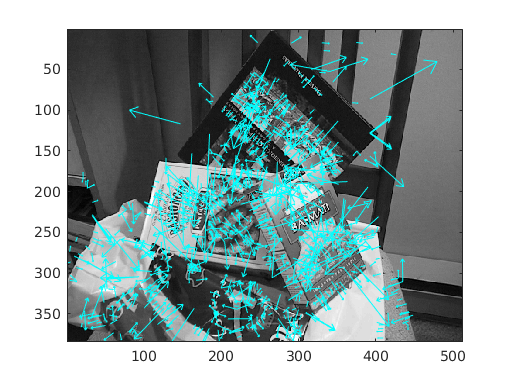
\includegraphics[width=.7\textwidth]{keypoints.png}
 \caption{Found keypoints in `scene.pgm' using SIFT.}
 \label{fig1}
\end{figure}

Figure \ref{fig2} shows the matches between the two images. The script reports 98 matches. This corresponds to $98/882 = 11.11\%$ of the keypoints found in `book.pgm' matched with $98/1021 = 9.60\%$ of the keypoints found in the `scene.pgm'. Not all matches are correct. We observe for example that the match found with the upper left corner of the small image is incorrect, but it is reasonable, since both of the keypoints are found in a square corner of a gray area with a black background. Another example is the match found between the lower left corner of the Basmati rice pack and an area on the illustration on the book. This match is reasonable to the extent of the pixels looking similar, but not in respect of the context, which is clearly different; a human can easily distinguish the contexts (one keypoint is localized in an illustration, whereas the other one is part of a rice pack).

\begin{figure}[H]
 \centering
 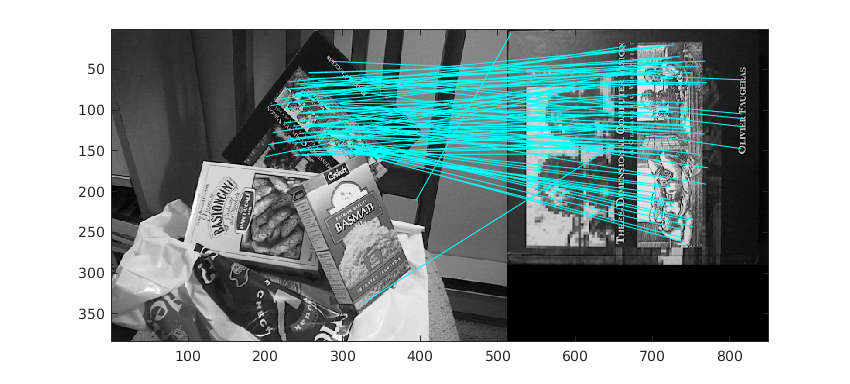
\includegraphics[width=1\textwidth]{matches.png}
 \caption{Matches between `scene.pgm' and `book.pgm' using SIFT.}
 \label{fig2}
\end{figure}

Figure \ref{fig3} shows the matches between the two images. The script reports 98 matches. This corresponds to $34/579 = 5.87\%$ of the keypoints found in `book.pgm' matched with $34/1021 = 3.33\%$ of the keypoints found in the `scene.pgm'. Again not all matches are correct. There is one clearly incorrect match between the top of the basmati pack and the edge between the chair and wall. This match is quite reasonable, since the gray color of the wall and pack are similar, just as the color of the chair and background in `basmati.pgm'. Moreover in both cases the edge is close to a straight line.
\begin{figure}[H]
 \centering
 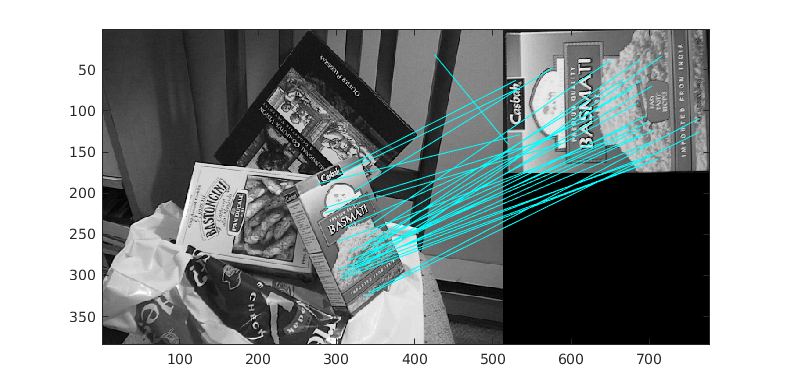
\includegraphics[width=1\textwidth]{matches2.png}
 \caption{Matches between `scene.pgm' and `basmati.pgm' using SIFT.}
 \label{fig3}
\end{figure}

Table \ref{table1} shows a comparison between the two street images when matched with the five detail images. In `streetlarge.png' 5316 keypoints are found and in `street.png' 1452, so the number is much higher in the higher resolution image. Table \ref{table1} shows that also the number of matches found is much higher for the higher resolution image. The table shows that the percentage of keypoints of the detail images that is matched is around 3 to 4 times as high for the high resolution image as it is for the lower resolution image. The percentage of keypoints of the street images that is matches is slightly higher for the lower resolution street image.

Even though the number of found matches is much higher for the high resolution image, the percentage of mismatches is also a lot higher for all images except for `detail1.png'. This shows that a higher resolution image does not always improve the match. This has to do with the fact that in a high resolution image, more details are given. Details cause more keypoints to be found, but these keypoints only describe small textures that do not contribute to matching the object in general. Instead they can cause faulty matches, since they cause more contrasting pixels.

\begin{table}[H]
 \centering
 \caption{Matches ($m$), mismatches ($mism$) and matches $/$ keypoints ($k$) between `street.png' and `streetlarge.png' and the five details. Mismatches were hard to distinguish exactly, so the table gives the lower bound of the mismatch percentages.}
 \label{table1}
 \begin{tabular}{|c|c|c|c|c||c|c|c|c|}
 \hline
 & \multicolumn{4}{c||}{Street small} & \multicolumn{4}{c|}{Street large} \\
 \hline
  Detail & $m$ & $m/k$ (detail) & $m/k$(street) & $mism$ & $m$ & $m/k$ (detail) & $m/k$(street) & $mism$ \\
  \hline
  1 & 25 & $1.57\%$ & $1.72\%$ & $4\%$ & 82 & $5.15\%$ & $1.54\%$ & $3.66\%$ \\
  2 & 6 & $13.04\%$ & $0.41\%$ & $0\%$ & 17 & $36.96\%$ & $0.32\%$ & $23.53\%$ \\
  3 & 37 & $6.29\%$ & $2.55\%$ & $0\%$ & 110 & $18.71\%$ & $2.07\%$ & $21.82\%$ \\
  4 & 20 & $5.43\%$ & $1.38\%$ & $10\%$ & 73 & $19.84\%$ & $1.37\%$ & $21.92\%$ \\
  5 & 6 & $4.76\%$ & $0.41\%$ & $16.67\%$ & 17 & $14.49\%$ & $0.32\%$ & $47.06\%$ \\
  \hline
 \end{tabular}
\end{table}

\subsection{}
Tables \ref{table2} and \ref{table3} show the matches between the outdoor detail images and the indoor scene image and vice versa. In both of the situations a small number of matches is found, which is logical because the details are not present in the scenic images, which essentially makes every match a mismatch. 

It would not be advisable to use a threshold using the absolute number of matches, because that would depend heavily on the pictures themselves. Sometimes an image has many keypoints, making many matches possible, but in other instances an image has few keypoints, limiting the number of possible matches. Therefore looking at the percentage of matches of keypoints would be a better measure to use. 

Looking at the statistics, a threshold of the percentage might be possible. However, this would be impossible using the percentage of the larger image (the scene), since it differs per scenic image how much of its keypoints are made up out of the specific object you want to match, resulting in a difference of percentages per scene image. It would therefore be logical to use the percentage of the smaller image for the threshold (under the assumption that this just contains the object we want to match). Of course we would need more data to properly set a threshold, but looking at the column `$m/k$ (detail) (\%)' and the data in table \ref{table1}, a threshold of somewhere around 1 \% might be in order for situations in which you would not want false negatives, for example in the case of diagnosing a patient. Using this threshold, detail 4 in table \ref{table2} would be falsely classified as a match, but the other details would be correctly classified. On the other hand if false positives would be disfavoured, the threshold would have to be set higher, for example at 6 \%.

\begin{table}[H]
\centering
 \caption{Matches found between the outdoor detail images and the indoor scene image.}
 \label{table2}
 \begin{tabular}{|c|c|c|c|}
 \hline
  Detail & $m$ & $m/k$ (detail) ($\%$) & $m/k$(scene)($\%$) \\
  \hline
  1 & 1 & 0.06 & 0.10 \\
  2 & 0 & 0 & 0 \\
  3 & 0 & 0 & 0 \\
  4 & 2 & 5.4 & 0.20 \\
  5 & 0 & 0 & 0 \\
  \hline
 \end{tabular}
\end{table}

\begin{table}[H]
\centering
 \caption{Matches found between the indoor detail images and the outdoor scene image.}
 \label{table3}
 \begin{tabular}{|c|c|c|c||c|c|c|}
 \hline
 & \multicolumn{3}{c||}{Street small} & \multicolumn{3}{c|}{Street large} \\
 \hline
  Detail & $m$ & $m/k$ (detail) ($\%$) & $m/k$(street) ($\%$) & $m$ & $m/k$ (detail) ($\%$) & $m/k$(street) ($\%$) \\
  \hline
  Book & 1 & 0.11 & 0.07 & 6 & 0.68 & 0.11 \\
  Basmati & 1 & 0.17 & 0.07 & 3 & 0.52 & 0.06 \\
  \hline
 \end{tabular}
\end{table}

\subsection{}
Table \ref{table4} shows the data for the rotated book images matched to the scene image. The distribution of matches has a mean of 101.10 and a standard deviation of approximately 4.01. So the number of matches deviates little from the mean for different rotations of the image. Furthermore we can see that the percentages of number of matches in the keypoints remain approximately stable, as well as the number of mismatches which remains quite low with a maximum of 3, corresponding to a maximum of $3/98 \approx 0.03 \% $ of the total number of matches). All this suggests that the degree in which SIFT is rotation invariant is quite high, although not perfect.

\begin{table}[H]
\centering
 \caption{Matches found between the rotated book images and the indoor scene image.}
 \label{table4}
 \begin{tabular}{|c|c|c|c|c|}
 \hline
  Rotation & $m$ & $m/k$ (detail) ($\%$) & $m/k$(scene)($\%$) & $mism$\\
  \hline
  0 & 98 & 11.11 & 9.60 & 2 \\
  10 & 102 & 10.01 & 9.99 & 1 \\
  20 & 95 & 9.35 & 9.30 & 0 \\
  30 & 107 & 10.38 & 10.48 & 2 \\
  40 & 101 & 9.57 & 9.89 & 2 \\
  50 & 100 & 9.48 & 9.79 & 2 \\
  60 & 102 & 9.69 & 9.99 & 1 \\
  70 & 102 & 10.01 & 9.99 & 1 \\
  80 & 107 & 10.27 & 10.48 & 2 \\
  90 & 103 & 11.39 & 10.09 & 0 \\
  180 & 98 & 10.80 & 9.60 & 1 \\
  270 & 98 & 10.71 & 9.60 & 3 \\
  \hline
 \end{tabular}
\end{table}

\subsection{}


%\begin{appendices}
%\section{Code}
% %\lstinputlisting[caption={circorr},label={code:1a}]{../code/circorr.m}
%\end{appendices}
\end{document}
